\section{The logit model of demand}\label{sec:07-logit}

The logit is the simplest discrete choice model that delivers market demand for many differentiated products
from a handful of parameters. This section states its assumptions and derives its shares, elasticities and
diversion ratios. It then shows how the independence of the taste shocks restricts substitution. It closes
with estimation from individual choices, the setting in which \citet{McFadden1974} introduced the model.

\subsection{Setup and assumptions}\label{sec:07-logit-setup}

We observe markets $t = 1, \dots, T$. A market is a time period, a geographic area, or both. Market $t$
offers the inside products $j \in \mathcal{J}_t = \{1, \dots, J_t\}$ and an \emph{outside good} $j = 0$,
which stands for buying none of the inside products. A measure $M_t$ of consumers, the \emph{market size},
chooses among these $J_t + 1$ options. We interpret $M_t$ as the number of potential buyers. It is rarely
observed, so the researcher must choose it, and \cref{sec:07-market-size} studies the consequences of that
choice. Product $j$ in market $t$ has observed characteristics $x_{jt}$ (a $1 \times K$ row vector), a price
$p_{jt}$, and an \emph{unobserved product characteristic} $\xi_{jt}$.

\begin{assumption}[Logit demand]\label{asm:07-logit}
\leavevmode
\begin{enumerate}[label=(\roman*)]
  \item Each consumer $i$ in market $t$ buys one unit of exactly one option $j \in \{0\} \cup \mathcal{J}_t$,
  the option that gives her the highest utility.
  \item Utility is $u_{ijt} = \delta_{jt} + \epsilon_{ijt}$ for $j \in \mathcal{J}_t$ and
  $u_{i0t} = \epsilon_{i0t}$ for the outside good.
  \item The \emph{mean utility} is $\delta_{jt} = x_{jt}\beta - \alpha p_{jt} + \xi_{jt}$, with $\alpha > 0$.
  \item The shocks $\epsilon_{ijt}$ are independent across consumers, options and markets. Each has the
  type-I extreme value (Gumbel) distribution with CDF $F(\epsilon) = \exp(-e^{-\epsilon})$. The shocks are
  independent of $(x_t, p_t, \xi_t)$.
  \item Consumers and firms observe $\xi_{jt}$. The econometrician does not.
\end{enumerate}
\end{assumption}

Part (iii) contains a quasi-linear utility over income. Let consumer $i$ have income $y_i$, utility
$\alpha(y_i - p_{jt}) + x_{jt}\beta + \xi_{jt} + \epsilon_{ijt}$ from product $j$, and utility
$\alpha y_i + \epsilon_{i0t}$ from the outside good. The term $\alpha y_i$ is common to all options, so it
drops out of every comparison, and the model reduces to parts (ii) and (iii). The coefficient $\alpha$ is the
marginal utility of income. It converts utils into dollars. Quasi-linearity rules out income effects, a
restriction we revisit in \cref{sec:07-iia}. Part (i) rules out the purchase of several units or several
products, which \citet{Hendel1999} relaxes (\cref{sec:07-hendel}).

The unobserved characteristic $\xi_{jt}$ collects everything about product $j$ that consumers value and the
econometrician does not measure. \citet[p.~243]{Berry1994} mentions style, perceived quality, durability,
status and service at the point of sale. The term plays three roles. It is the demand shock of the model, the
analogue of the error in a homogeneous-goods demand curve. It lets the model fit the observed shares exactly,
as \cref{sec:07-inversion} shows. Finally, firms observe $\xi_{jt}$ when they set prices, so prices respond to
it, which makes them endogenous (\cref{sec:07-endogeneity}).

The shock $\epsilon_{ijt}$ admits several readings. It may capture characteristics of the consumer or of the
product that the econometrician does not observe. It may reflect measurement error or approximation error in
the utility function. It may also represent psychological biases or mistakes. \citet[p.~1412]{McFadden1984}
contrasts factors known to the decision maker but not to the observer with a random element in the decision
protocol itself. He notes that choice data cannot ordinarily distinguish the two. The distinction matters for
welfare. If $\epsilon_{ijt}$ measures taste, the expected maximum utility counts it as a benefit. If it
measures mistakes, the same formula counts errors as gains (\cref{sec:07-welfare-caveats}).

We need $\epsilon_{ijt}$ for the same reason that a regression needs an error term. Without it, every
consumer in a market ranks the products by $\delta_{jt}$ alone and buys the product with the highest mean
utility. Such a deterministic model predicts that one product takes the whole market, which no data set shows.
The shock spreads consumers over all options and makes every predicted share interior.

Two normalizations are needed because choices reveal only the ranking of utilities. Adding a constant to
every utility leaves choices unchanged, so we set the mean utility of the outside good to zero. This is the
location normalization. Multiplying every utility by a positive number also leaves choices unchanged, so we
fix the variance of $\epsilon_{ijt}$ at $\frac{\pi^2}{6}$, the variance of the standard Gumbel. This is the
scale normalization. The coefficients $\beta$ and $\alpha$ are therefore measured in units of the scale of
the taste shock. Ratios such as $\frac{\beta_k}{\alpha}$, the dollar value of characteristic $k$, do not depend
on the normalization. \Cref{ch:discrete} develops both normalizations (\cref{prop:06-normalization}) and the
role of the outside good (\cref{sec:06-outside}). The outside good does more than fix the location. Without
it, demand depends only on differences in prices, so a general increase in inside prices cannot reduce
aggregate output \citep[p.~247]{Berry1994}. \citet{Berry1994} cites \citet{MorrisonWinston1986} as an example of
a model with this unfortunate feature.

\subsection{Choice probabilities and market shares}\label{sec:07-logit-shares}

\begin{proposition}[Logit shares]\label{prop:07-logit-shares}
Under \cref{asm:07-logit}, the probability that a consumer in market $t$ chooses option $j$, and hence the
market share of $j$, is
\begin{equation}\label{eq:07-logit-share}
  s_{jt} = \frac{e^{\delta_{jt}}}{1 + \sum_{k \in \mathcal{J}_t} e^{\delta_{kt}}} \quad (j \in \mathcal{J}_t),
  \qquad\qquad
  s_{0t} = \frac{1}{1 + \sum_{k \in \mathcal{J}_t} e^{\delta_{kt}}} .
\end{equation}
\end{proposition}

The proposition restates \cref{prop:06-logit} with $V_{ij} = \delta_{jt}$ for $j \in \mathcal{J}_t$, $V_{i0} = 0$
and $\sigma_\epsilon = 1$. \Cref{sec:06-logitprob} proves it twice, once by integrating over the Gumbel density and
once from the max-stability of the Gumbel distribution (\cref{lem:06-maxstable}). We write
$\Lambda_t = 1 + \sum_{k \in \mathcal{J}_t} e^{\delta_{kt}}$ for the common denominator, the \emph{inclusive sum}, so
that $s_{jt} = \frac{e^{\delta_{jt}}}{\Lambda_t}$ and $s_{0t} = \frac{1}{\Lambda_t}$. The ``1'' in the inclusive sum is
$e^{\delta_{0t}}$ with the outside good's mean utility normalized to zero.

\begin{remark}[What the extreme value assumption buys]\label{rem:07-gumbel}
The Gumbel distribution has one main virtue. It yields a closed form for the integral over the maximum of
utilities. Its density resembles a normal density skewed to the right. Choices depend only on differences of
shocks, and the difference of two independent Gumbel variables has the logistic distribution, which looks like a
normal with fatter tails. Logit and probit models with independent errors therefore fit data in similar ways.
The substantive restrictions of the logit come from the independence and additivity of the shocks
(\cref{sec:07-iia}). The Gumbel form adds tractability and little else.
\end{remark}

\begin{remark}[From probabilities to shares]\label{rem:07-continuum}
\Cref{prop:07-logit-shares} gives a choice probability. It equals the market share when the market has a
continuum of consumers, so that the law of large numbers holds exactly. With $M_t$ distinct consumers choosing
independently, the observed share is an average of $M_t$ Bernoulli draws and has variance
$\frac{s_{jt}(1 - s_{jt})}{M_t}$ \citep[footnote~4]{Berry1994}. \citet{Berry1994} treats the share equation
as exact, which amounts to a continuum of consumers. Shares computed from samples of consumers contain
sampling error, the subject of \cref{sec:07-market-size}.
\end{remark}

\begin{remark}[A representative consumer]\label{rem:07-representative}
The same shares solve the problem of a representative consumer who allocates one unit of consumption across
the options $j = 0, \dots, J$ to maximize $\sum_j \delta_j q_j - \sum_j q_j\ln q_j$, with $\delta_0 = 0$
\citep{AndersonDePalmaThisse1988, AndersonDePalmaThisse1992}. The entropy term expresses a taste for variety.
\Cref{ch:diffprod} develops this foundation and compares the logit with the constant elasticity of
substitution system.
\end{remark}

\subsection{Derivatives, elasticities and diversion}\label{sec:07-logit-elasticities}

Every substitution pattern of the logit follows from the derivatives of \eqref{eq:07-logit-share}. We drop the
market index throughout this subsection.

\begin{proposition}[Logit share derivatives]\label{prop:07-logit-derivs}
Under \cref{asm:07-logit}, for $j, k \in \mathcal{J}$ with $k \ne j$,
\begin{equation}\label{eq:07-logit-derivs-delta}
  \frac{\partial s_j}{\partial \delta_j} = s_j(1 - s_j), \qquad
  \frac{\partial s_j}{\partial \delta_k} = -s_j s_k, \qquad
  \frac{\partial s_0}{\partial \delta_k} = -s_0 s_k .
\end{equation}
Since $\frac{\partial \delta_j}{\partial p_j} = -\alpha$, the price derivatives are
\begin{equation}\label{eq:07-logit-derivs-price}
  \frac{\partial s_j}{\partial p_j} = -\alpha s_j(1 - s_j), \qquad
  \frac{\partial s_j}{\partial p_k} = \alpha s_j s_k, \qquad
  \frac{\partial s_0}{\partial p_k} = \alpha s_0 s_k .
\end{equation}
\end{proposition}

\begin{proof}
Write $s_j = \frac{e^{\delta_j}}{\Lambda}$ with $\Lambda = 1 + \sum_l e^{\delta_l}$, and note that
$\frac{\partial \Lambda}{\partial \delta_k} = e^{\delta_k}$. The quotient rule gives the own derivative:
\begin{equation*}
  \frac{\partial s_j}{\partial \delta_j}
  = \frac{e^{\delta_j}\Lambda - e^{\delta_j}e^{\delta_j}}{\Lambda^2}
  = \frac{e^{\delta_j}}{\Lambda} - \Big(\frac{e^{\delta_j}}{\Lambda}\Big)^2
  = s_j(1 - s_j).
\end{equation*}
For $k \ne j$ the numerator of $s_j$ does not depend on $\delta_k$, so only the denominator moves:
\begin{equation*}
  \frac{\partial s_j}{\partial \delta_k} = -\frac{e^{\delta_j}e^{\delta_k}}{\Lambda^2} = -s_j s_k .
\end{equation*}
The same step applied to $s_0 = \frac{1}{\Lambda}$ gives $\frac{\partial s_0}{\partial \delta_k} =
-\frac{e^{\delta_k}}{\Lambda^2} = -s_0 s_k$. The price derivatives follow from the chain rule, because $p_k$
enters only $\delta_k$, with coefficient $-\alpha$.
\end{proof}

\casehead{Elasticities}
Multiplying the price derivatives by $\frac{p_k}{s_j}$ gives the elasticities. Following the convention of this
book, we report the own-price elasticity as a positive number:
\begin{equation}\label{eq:07-logit-elast}
  \varepsilon_j = -\frac{\partial s_j}{\partial p_j}\frac{p_j}{s_j} = \alpha p_j(1 - s_j), \qquad
  \varepsilon_{jk} = \frac{\partial s_j}{\partial p_k}\frac{p_k}{s_j} = \alpha p_k s_k, \qquad
  \varepsilon_{0k} = \frac{\partial s_0}{\partial p_k}\frac{p_k}{s_0} = \alpha p_k s_k .
\end{equation}
Since $q_j = M s_j$ and $M$ does not depend on prices, quantity elasticities equal share elasticities. The cross
elasticity $\varepsilon_{jk}$ does not depend on $j$. Arrange the elasticities in a matrix whose rows index the
option whose demand responds and whose columns index the product whose price changes. Every off-diagonal entry
of column $k$ equals $\alpha p_k s_k$, and so does the entry of the outside good. A rise in $p_k$ therefore
raises the demand for every other option, inside or outside, by the same percentage. Some studies report
\emph{semi-elasticities}, the percentage change in a share per unit change in a price,
$100\,\frac{\partial s_j}{\partial p_k}\frac{1}{s_j}$. In the logit these equal $-100\,\alpha(1 - s_j)$ on the
diagonal and $100\,\alpha s_k$ off it. \Cref{ch:blp} reads a table of semi-elasticities from
\citet{BerryLevinsohnPakes1995} in these units.

\casehead{Diversion ratios}
The \emph{diversion ratio} $D_{jk}$ is the fraction of the sales that product $j$ loses after a small increase in
its own price that goes to option $k$. By \cref{prop:07-logit-derivs},
\begin{equation}\label{eq:07-logit-diversion}
  D_{jk} = -\frac{\frac{\partial s_k}{\partial p_j}}{\frac{\partial s_j}{\partial p_j}}
  = \frac{\alpha s_j s_k}{\alpha s_j(1 - s_j)} = \frac{s_k}{1 - s_j}, \qquad
  D_{j0} = \frac{\alpha s_j s_0}{\alpha s_j(1 - s_j)} = \frac{s_0}{1 - s_j} .
\end{equation}
The ratios sum to one over the options other than $j$, because the shares of those options sum to $1 - s_j$.
Consumers who leave $j$ spread over the remaining options in proportion to their shares, whatever the
similarity of those options to $j$. Diversion ratios measure how closely two products compete. They drive the
upward pricing pressure of a merger, so \eqref{eq:07-logit-diversion} reappears in \cref{ch:mergers}.

\casehead{The category elasticity}
Market definition asks how demand for a group of products responds when all of their prices rise together.
Raise every inside price by the same amount $\Delta$, so that every mean utility falls by $\alpha\Delta$. Let
$E = \sum_{k \in \mathcal{J}} e^{\delta_k}$ denote the inside sum at $\Delta = 0$. The total inside share and
its logarithm are
\begin{equation*}
  1 - s_0(\Delta) = \frac{e^{-\alpha\Delta}E}{1 + e^{-\alpha\Delta}E}, \qquad
  \ln\big(1 - s_0(\Delta)\big) = -\alpha\Delta + \ln E - \ln\big(1 + e^{-\alpha\Delta}E\big).
\end{equation*}
Differentiate with respect to $\Delta$ and evaluate at $\Delta = 0$:
\begin{equation}\label{eq:07-category-semi}
  \frac{\dd\ln(1 - s_0)}{\dd\Delta}
  = -\alpha + \alpha\,\frac{E}{1 + E}
  = -\alpha + \alpha(1 - s_0)
  = -\alpha s_0 .
\end{equation}
For a proportional increase $p_k \mapsto (1 + \lambda)p_k$ of every inside price, each mean utility moves at the
rate $\frac{\partial \delta_k}{\partial \lambda} = -\alpha p_k$. Writing $\ln(1 - s_0) = \ln E - \ln\Lambda$
and differentiating at $\lambda = 0$,
\begin{align}
  \frac{\dd\ln(1 - s_0)}{\dd\lambda}
  &= \sum_{k}\frac{e^{\delta_k}}{E}(-\alpha p_k) - \sum_{k}\frac{e^{\delta_k}}{\Lambda}(-\alpha p_k)
   = -\alpha\sum_k p_k s_k\Big(\frac{1}{1 - s_0} - 1\Big) \notag\\
  &= -\alpha s_0\sum_k \frac{s_k}{1 - s_0}\,p_k
   = -\alpha s_0\,\bar p, \label{eq:07-category-elast}
\end{align}
where $\bar p$ is the share-weighted average inside price. The category elasticity is proportional to the
outside share. When few consumers choose the outside good, the inside products as a group face inelastic
demand, even if each of them faces elastic demand. A hypothetical monopolist of all inside products would then
raise prices, which is the logic of the hypothetical monopolist test in \cref{ch:mergers}. Since $s_0$
depends on the assumed market size, so does the category elasticity (\cref{sec:07-market-size}).

\begin{example}[An illustrative logit market]\label{ex:07-logit-numbers}
Consider one market with four inside products, $\alpha = 1$, mean utilities $\delta = (1.0, 0.5, 0.1,
-0.5)$ and prices $p = (2.0, 2.5, 3.0, 4.0)$. The implied non-price utility $x_j\beta + \xi_j = \delta_j +
\alpha p_j$ equals $(3.0, 3.0, 3.1, 3.5)$, so the expensive products are somewhat better.
\Cref{tab:07-logit-elast} reports the shares, the elasticity matrix and the diversion ratios, computed by
\texttt{figures/ch07/src/logit\_example.py}. Three features stand out. Own elasticities rise with price, from
1.23 for the cheapest product to 3.66 for the most expensive one. Each column of cross elasticities is
constant and equals the outside-good entry, for example $\alpha p_1 s_1 = 2.0 \times 0.384 = 0.768$ in column
1. When any of products 2 to 4 raises its price, the largest share of its lost sales goes to product 1, the
largest product. Product 1's own lost sales go mostly to product 2, the next largest. The category elasticities are $\alpha s_0 = 0.141$ per unit of common price increase and
$\alpha s_0\bar p = 0.356$ for a proportional increase. The category faces inelastic demand while every
product faces elastic demand.
\end{example}

\begin{table}[htbp]
\centering
\caption{Shares, price elasticities and diversion ratios in an illustrative logit market}
\label{tab:07-logit-elast}
\begin{tabular}{@{}lcccccc@{}}
\toprule
\multicolumn{7}{@{}l}{\textit{Panel A. Price elasticities $\varepsilon_{jk}$}} \\
 & & & \multicolumn{4}{c}{Product $k$ whose price changes} \\
\cmidrule(l){4-7}
Option $j$ & $p_j$ & $s_j$ & 1 & 2 & 3 & 4 \\
\midrule
1 & 2.0 & 0.384 & $-1.232$ & 0.582 & 0.468 & 0.343 \\
2 & 2.5 & 0.233 & 0.768 & $-1.918$ & 0.468 & 0.343 \\
3 & 3.0 & 0.156 & 0.768 & 0.582 & $-2.532$ & 0.343 \\
4 & 4.0 & 0.086 & 0.768 & 0.582 & 0.468 & $-3.657$ \\
0 (outside) & & 0.141 & 0.768 & 0.582 & 0.468 & 0.343 \\
\midrule
\multicolumn{7}{@{}l}{\textit{Panel B. Diversion ratios $D_{jk}$}} \\
 & \multicolumn{6}{c}{Option $k$ receiving the diverted sales} \\
\cmidrule(l){2-7}
Product $j$ & & 0 & 1 & 2 & 3 & 4 \\
\midrule
1 & & 0.229 & & 0.378 & 0.253 & 0.139 \\
2 & & 0.184 & 0.501 & & 0.204 & 0.112 \\
3 & & 0.167 & 0.455 & 0.276 & & 0.102 \\
4 & & 0.155 & 0.420 & 0.255 & 0.171 & \\
\bottomrule
\end{tabular}

\vspace{4pt}
\begin{minipage}{0.86\textwidth}
\footnotesize Notes: $\alpha = 1$, $\delta = (1.0, 0.5, 0.1, -0.5)$. Panel A: entry $(j, k)$ is
$\frac{\partial s_j}{\partial p_k}\frac{p_k}{s_j}$, so own elasticities appear on the diagonal as negative
numbers. Panel B: entry $(j, k)$ is $D_{jk} = \frac{s_k}{1 - s_j}$, and each row sums to one. Computed by
\texttt{figures/ch07/src/logit\_example.py}.
\end{minipage}
\end{table}

\subsection{Independence of irrelevant alternatives}\label{sec:07-iia}

\begin{definition}[IIA]\label{def:07-iia}
A system of choice probabilities $P(j \mid C)$, defined for every choice set $C$, satisfies
\emph{independence of irrelevant alternatives} (IIA) if, for all $j, k \in A \subseteq C$,
\begin{equation*}
  \frac{P(j \mid C)}{P(k \mid C)} = \frac{P(j \mid A)}{P(k \mid A)} .
\end{equation*}
The ratio must also not depend on the characteristics of the alternatives other than $j$ and $k$.
\end{definition}

\citet{Luce1959} took IIA as an axiom of probabilistic choice. The logit satisfies it, since
\eqref{eq:07-logit-share} gives
\begin{equation}\label{eq:07-logit-iia}
  \frac{s_j}{s_k} = e^{\delta_j - \delta_k},
\end{equation}
which involves only $j$ and $k$. \Cref{sec:06-gev} relates the axiom to the Gumbel distribution.

\casehead{The red bus and the blue bus}
\citet{Debreu1960} objected to Luce's axiom with an example of two nearly identical alternatives. The standard
version concerns commuting \citep[Section~3.3.2, p.~46]{Train2009}.
A commuter chooses between a car and a red bus with
equal mean utilities $v$, so each has probability $\frac{1}{2}$. Now add a blue bus, identical to the red bus
except for its color. The logit gives
\begin{equation*}
  P_{\text{car}} = P_{\text{red}} = P_{\text{blue}} = \frac{e^{v}}{3e^{v}} = \frac{1}{3} .
\end{equation*}
IIA requires $\frac{P_{\text{car}}}{P_{\text{red}}} = 1$ to survive the new option, so the blue bus draws riders
from the car and from the red bus in equal proportions. Common sense says the blue bus draws riders only from
the red bus, giving the probabilities $(\frac{1}{2}, \frac{1}{4}, \frac{1}{4})$. The logit also predicts
that painting some buses blue raises the total bus share from $\frac{1}{2}$ to $\frac{2}{3}$.
\Cref{sec:07-nl-substitution} shows how the nested logit repairs the example (\cref{fig:07-redbus}).

\casehead{Implications for demand}
IIA has three consequences for a demand system. The first is substitution in proportion to shares, through
\eqref{eq:07-logit-diversion}. Suppose the price of a BMW 7-series rises. The logit sends its buyers to a Mazda
323 and to a Lexus LS400 in proportion to their shares, so the small car, which sells more, gains more.
\citet[p.~847]{BerryLevinsohnPakes1995} make the point with a Yugo and a Mercedes that have the same share.
The two cars must then have the same cross-price derivative with respect to any third car. A rise in the BMW
price therefore raises the demand for Yugos and for Mercedes equally. \citet[p.~523]{Nevo2000a} gives a cereal
version. If Cap'n Crunch, a children's cereal, and Grape Nuts, a nutrition cereal, have similar shares, a rise
in the price of Lucky Charms, another children's cereal, diverts equally to both.

The second consequence concerns own elasticities. With small shares, $\varepsilon_j = \alpha p_j(1 - s_j)
\approx \alpha p_j$, so own elasticities rise almost in proportion to price (\cref{fig:07-logit-demand}).
Expensive products face the most elastic demand. This runs against the intuition that buyers of expensive
products are less sensitive to price. Under single-product Bertrand pricing the Lerner index equals
$\frac{1}{\varepsilon_j}$, so cheaper products must carry higher percentage markups.
\citet[p.~522]{Nevo2000a} notes that this requires cheaper brands to have lower marginal costs as a percentage
of price, which need not hold.

The third consequence concerns markups. A single-product firm facing logit demand sets the dollar markup
$p_j - mc_j = \frac{1}{\alpha(1 - s_j)}$ (\cref{sec:07-supply}). Two products with the same share carry the
same markup, whatever their characteristics. \citet[p.~847]{BerryLevinsohnPakes1995} illustrate with a Jaguar
and a Yugo of equal share, which must have the same own-price derivative and hence the same markup.

\begin{figure}[htbp]
\centering
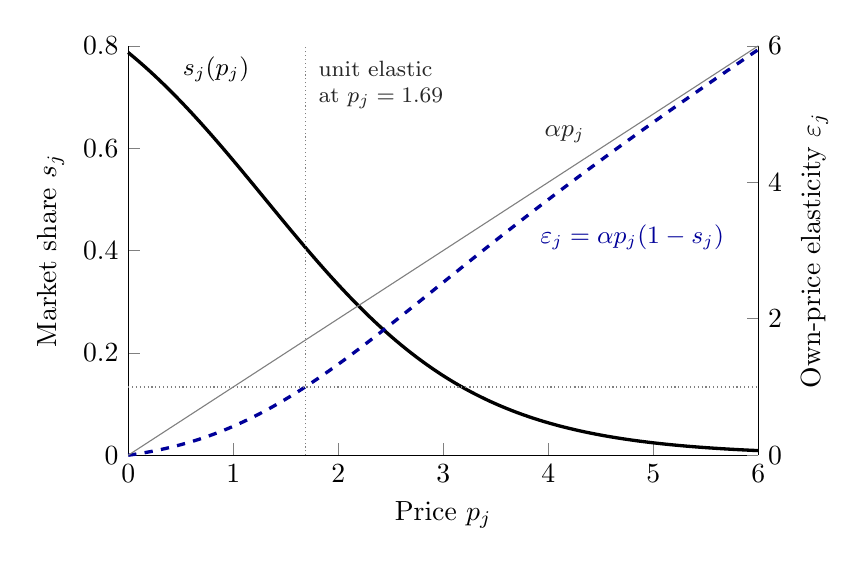
\begin{tikzpicture}
\begin{axis}[
  scale only axis, width=0.66\textwidth, height=5.2cm,
  xmin=0, xmax=6, ymin=0, ymax=0.8,
  axis y line*=left, axis x line*=bottom,
  xlabel={Price $p_j$}, ylabel={Market share $s_j$},
  ytick={0,0.2,0.4,0.6,0.8},
  yticklabel style={/pgf/number format/fixed, /pgf/number format/precision=1},
  clip=false]
  \addplot[very thick, black, samples=121, domain=0:6] {exp(2-x)/(2+exp(2-x))}
    node[pos=0.07, above right, font=\small] {$s_j(p_j)$};
  \draw[densely dotted, gray] (axis cs:1.685,0) -- (axis cs:1.685,0.8);
  \node[font=\footnotesize, anchor=north west, gray!30!black, align=left] at (axis cs:1.72,0.79)
    {unit elastic\\ at $p_j = 1.69$};
\end{axis}
\begin{axis}[
  scale only axis, width=0.66\textwidth, height=5.2cm,
  xmin=0, xmax=6, ymin=0, ymax=6,
  axis y line*=right, axis x line=none,
  ylabel={Own-price elasticity $\varepsilon_j$},
  clip=false]
  \addplot[very thick, dashed, blue!60!black, samples=121, domain=0:6] {x*(1 - exp(2-x)/(2+exp(2-x)))}
    node[pos=0.62, below right, font=\small] {$\varepsilon_j = \alpha p_j(1 - s_j)$};
  \addplot[thin, gray, domain=0:6] {x} node[pos=0.74, above left, font=\small, gray!30!black] {$\alpha p_j$};
  \addplot[densely dotted, gray, domain=0:6] {1};
\end{axis}
\end{tikzpicture}
\caption{Logit demand and its own-price elasticity. The solid curve (left axis) is the share of one product,
$s_j = \frac{e^{2 - p_j}}{2 + e^{2 - p_j}}$, holding the other options fixed, with $\alpha = 1$. The dashed
curve (right axis) is the own-price elasticity $\alpha p_j(1 - s_j)$, which approaches the line $\alpha p_j$ as
the share falls. The dotted horizontal line marks an elasticity of one.}
\label{fig:07-logit-demand}
\end{figure}

\casehead{The source of the restriction}
A consumer buys product $j$ either because $\delta_j$ is high or because her shock $\epsilon_{ij}$ is high.
When $p_j$ rises, the consumers who leave $j$ are those whose shock $\epsilon_{ij}$ was just large enough to make
$j$ their choice. Their shocks for the other products are independent of $\epsilon_{ij}$. Their second choices
therefore follow the same distribution as the first choices of the population, which is the vector of market
shares \citep[p.~523]{Nevo2000a}. \citet[p.~246]{Berry1994} stresses that the restriction comes from the i.i.d.
additive error. Whenever tastes vary only through such an error, the mean utilities $\delta_j$ determine shares
and elasticities. Two products with the same shares then have the same cross elasticity with any third product,
whatever the distribution of the error (\cref{rem:07-berry-iid} gives the argument). An independent probit has
the same problem, which led \citet{HausmanWise1978} to allow correlated errors.

The cure is correlation of utility across similar products. The nested logit (\cref{sec:07-nested}) builds the
correlation into the shock. Random coefficients (\cref{ch:blp}) generate it from heterogeneous tastes for
characteristics. Both remedies add heterogeneity across consumers. A different distribution for an
independent shock would leave the problem in place. \citet[pp.~1414--1415]{McFadden1984} adds a related point.
IIA follows from letting the utility of $j$ depend only on the attributes of $j$. If utilities may depend on the
attributes of all alternatives, the logit form can approximate any continuous choice model
(\cref{rem:06-universal}). The restriction lies in the specification of utility, and the logistic function
plays no part in it.

\casehead{Other functional forms for price}
The elasticity pattern also reflects the linearity of utility in price. Suppose utility depends on the
logarithm of price, $\delta_j = x_j\beta - \alpha\ln p_j + \xi_j$. Then $\frac{\partial \delta_j}{\partial p_j} =
-\frac{\alpha}{p_j}$ and
\begin{equation*}
  \frac{\partial s_j}{\partial p_j} = -\frac{\alpha}{p_j}\,s_j(1 - s_j), \qquad
  \varepsilon_j = \alpha(1 - s_j),
\end{equation*}
which is nearly constant across products \citep[pp.~522--523]{Nevo2000a}. \citet{BjornerstedtVerboven2016}
compare a unit-demand nested logit, linear in price, with a constant-expenditure version. In the latter, price
enters in logarithms and a buyer spends a constant fraction of income on the chosen product (eq.~(3), p.~139).
For Swedish analgesics in December 2008, their nested logit models give average brand-level own elasticities of
2.43 under constant expenditure and 8.84 under unit demand (Table~6, p.~147). The difference has large consequences
for predicted merger effects (\cref{ch:mergers}).
\citet[p.~231]{AskerNocke2021} list the paper among the ex-post evaluations of the accuracy of merger simulation.
Either way, the functional form decides how own elasticities vary across products before any data are used.

Income effects require leaving the quasi-linear form. With $u_{ij} = \alpha\ln(y_i - p_j) + x_j\beta + \xi_j +
\epsilon_{ij}$, income no longer cancels, and the marginal utility of money $\frac{\alpha}{y_i - p_j}$ varies
across consumers. Market shares become averages of logit probabilities over the income distribution of the
market. This is a random coefficients model, and its shares must be simulated (\cref{ch:blp}).

\begin{remark}[Adequacy depends on the use]\label{rem:07-adequacy}
Whether the logit is good enough cannot be judged in isolation. If a question does not hinge on the matrix of
cross elasticities, the logit may serve well. \citet{Einav2007} uses a nested logit without prices to separate
seasonal swings in the demand for movies from seasonal swings in the number and quality of releases
(\cref{sec:07-einav}). The same model would be a poor basis for merger simulation, which depends on the
cross elasticities between close substitutes.
\end{remark}

\subsection{Logit with individual data: maximum likelihood}\label{sec:07-micro-ml}

The logit began as a model of individual choice. \citet{McFadden1974} introduced the \emph{conditional
logit}, in which choice probabilities depend on attributes of the alternatives, and studied its maximum
likelihood estimator. Individual data let us interact product characteristics with consumer attributes, which
relaxes IIA across consumer types.

\casehead{The conditional logit with consumer attributes}
Suppose we observe in each market $t$ a sample $\mathcal{I}_t$ of consumers, their attributes $D_i$ (an
$R$-vector), and their choices $y_{ijt} \in \{0, 1\}$. Let
\begin{equation}\label{eq:07-micro-utility}
  u_{ijt} = \delta_{jt} + \sum_{k=1}^{K}\sum_{r=1}^{R} x_{jkt}\pi_{kr}D_{ir} + \epsilon_{ijt}, \qquad
  u_{i0t} = \epsilon_{i0t},
\end{equation}
with $\epsilon_{ijt}$ as in \cref{asm:07-logit}. The terms $\delta_{jt}$ are \emph{alternative-specific
constants}, one for each product and market. They absorb $x_{jt}\beta - \alpha p_{jt} + \xi_{jt}$ in full. The
coefficients $\pi_{kr}$ let consumers with different attributes value characteristics differently. Collect the
parameters in $\theta = (\delta, \pi)$. Write the deterministic utility as $V_{ijt} = w_{ijt}\theta$, where the
row vector $w_{ijt}$ contains a dummy for the pair $(j, t)$ and the interactions $x_{jkt}D_{ir}$, and set
$w_{i0t} = 0$. The choice probabilities and the log-likelihood are
\begin{equation}\label{eq:07-micro-ll}
  P_{ijt}(\theta) = \frac{e^{w_{ijt}\theta}}{\sum_{k=0}^{J_t} e^{w_{ikt}\theta}}, \qquad
  \ell(\theta) = \sum_{t=1}^{T}\sum_{i \in \mathcal{I}_t}\sum_{j=0}^{J_t} y_{ijt}\ln P_{ijt}(\theta) .
\end{equation}

\begin{proposition}[Global concavity]\label{prop:07-ml-concave}
The log-likelihood in \eqref{eq:07-micro-ll} is concave in $\theta$. It is strictly concave if the matrix that
stacks the rows $w_{ijt}$, over all sampled consumers $i$, all $j \in \mathcal{J}_t$ and all $t$, has full
column rank. A stationary point of $\ell$ is then its unique global maximum.
\end{proposition}

\begin{proof}
Fix a consumer $i$ in market $t$ and drop the index $t$. Since $\sum_j y_{ij} = 1$, her contribution to the
log-likelihood is
\begin{equation*}
  \ell_i(\theta) = \sum_j y_{ij}w_{ij}\theta - \ln\sum_k e^{w_{ik}\theta} .
\end{equation*}
The first term is linear in $\theta$. Differentiating once,
\begin{equation*}
  \frac{\partial \ell_i}{\partial \theta}
  = \sum_j y_{ij}w_{ij}^\T - \sum_k P_{ik}w_{ik}^\T
  = \sum_j (y_{ij} - P_{ij})\,w_{ij}^\T .
\end{equation*}
Let $\bar w_i = \sum_k P_{ik}w_{ik}$ be the probability-weighted mean of the rows. The probabilities satisfy
$\frac{\partial P_{ik}}{\partial \theta^\T} = P_{ik}(w_{ik} - \bar w_i)$. Differentiating a second time,
\begin{equation*}
  \frac{\partial^2 \ell_i}{\partial \theta\,\partial \theta^\T}
  = -\sum_k P_{ik}\,w_{ik}^\T(w_{ik} - \bar w_i)
  = -\sum_k P_{ik}\,(w_{ik} - \bar w_i)^\T(w_{ik} - \bar w_i),
\end{equation*}
where the second equality subtracts $\bar w_i^\T\sum_k P_{ik}(w_{ik} - \bar w_i) = 0$. For any vector $v$,
\begin{equation*}
  v^\T\,\frac{\partial^2 \ell_i}{\partial \theta\,\partial \theta^\T}\,v
  = -\sum_k P_{ik}\big[(w_{ik} - \bar w_i)v\big]^2 \le 0 .
\end{equation*}
The right side is minus the variance of $w_{ik}v$ when $k$ is drawn with probabilities $P_{ik}$. Summing over
consumers shows that the Hessian of $\ell$ is negative semidefinite at every $\theta$, so $\ell$ is concave.

For strict concavity, suppose that $v^\T\nabla^2\ell(\theta)v = 0$. Every $P_{ik}$ is positive, so
$(w_{ik} - \bar w_i)v = 0$ for all $i$ and $k$. Then $w_{ik}v$ takes the same value for every option $k$ of
consumer $i$, and that value is $w_{i0}v = 0$. Hence $w_{ijt}v = 0$ for every row of the stacked matrix, and
the rank condition gives $v = 0$. A strictly concave function has at most one maximizer, and any stationary
point is that maximizer.
\end{proof}

\citet{McFadden1974} established this property, and \citet[p.~1413]{McFadden1984} restates it: barring linear
dependence of the explanatory variables, any stationary value is a global maximum. \Cref{eq:06-hessian}
derives the same Hessian in the notation of \cref{ch:discrete}. Concavity has practical value. Newton's method
with a line search, such as step-halving, converges to the maximum from any starting value. The estimate
therefore does not depend on where the search begins. Undamped Newton steps can still overshoot from poor
starting values. A maximum can
fail to exist when some combination of the regressors predicts the observed choices perfectly, as with
separation in a binary logit.

\casehead{Constants and shares}
The first-order condition for the constant $\delta_{jt}$ reads
\begin{equation}\label{eq:07-micro-foc}
  \frac{\partial \ell}{\partial \delta_{jt}} = \sum_{i \in \mathcal{I}_t}\big(y_{ijt} - P_{ijt}(\hat\theta)\big) = 0,
\end{equation}
so the average predicted probability of $j$ equals its sample share $\hat s_{jt}$. Without interactions
($\pi = 0$), every consumer in market $t$ has $P_{ijt} = \frac{e^{\delta_{jt}}}{1 + \sum_k e^{\delta_{kt}}}$, and
\eqref{eq:07-micro-foc} gives $\hat\delta_{jt} = \ln\hat s_{jt} - \ln\hat s_{0t}$. The maximum likelihood
estimates of the constants are the logit inversion of the sample shares, which \cref{sec:07-inversion-logit}
derives for market data.

\casehead{Micro data do not remove the need for instruments}
The constants absorb $\xi_{jt}$, so the likelihood in \eqref{eq:07-micro-ll} has no endogeneity problem. The
price coefficient, however, cannot be estimated from it. All consumers in a market face the same price, so
$p_{jt}$ is collinear with the dummy for $(j, t)$. The coefficients $\beta$ and $\alpha$ come from a second
step that regresses the estimated constants on characteristics and prices,
\begin{equation}\label{eq:07-micro-second}
  \hat\delta_{jt} = x_{jt}\beta - \alpha p_{jt} + \xi_{jt} + (\hat\delta_{jt} - \delta_{jt}) .
\end{equation}
This step compares products and markets. There $p_{jt}$ is correlated with $\xi_{jt}$ for the reasons given in
\cref{sec:07-endogeneity}, so the second step needs instruments, exactly as with market data
\citep[p.~259]{Berry1994}. Micro data reveal how tastes differ across consumers within a market, including
interactions of price with income. The average response to price still requires exogenous variation in
prices. \Cref{sec:08-micro-twostep} develops the two-step estimator with random coefficients, and \cref{ch:blp}
discusses \citet{Goldberg1995} and \citet*{BerryLevinsohnPakes2004}.

\casehead{Testing IIA}
IIA has a testable implication. Let $D$ be a subset of the full choice set $C$. If the logit is correct, the
probability of choosing $j$ given that the choice lies in $D$ is the logit $\frac{e^{V_{ij}}}{\sum_{k \in D}
e^{V_{ik}}}$, with the same parameters. We can therefore estimate the model on the consumers who chose an
alternative in $D$, treating $D$ as their choice set. This gives a consistent but inefficient estimator
$\hat\beta_D$ of the parameters that choices within $D$ identify. The full-sample estimator $\hat\beta_C$ is
consistent and efficient. If IIA fails,
the two estimators generally converge to different limits. Following the principle of \citet{Hausman1978},
the variance of the difference under the null is the difference of the variances, $\hat V_D - \hat V_C$. The
statistic
\begin{equation}\label{eq:07-hm-test}
  S = (\hat\beta_D - \hat\beta_C)^\T\,(\hat V_D - \hat V_C)^{-}\,(\hat\beta_D - \hat\beta_C),
\end{equation}
where $^{-}$ denotes a generalized inverse when the difference of the variances is singular. The statistic
is asymptotically chi-squared with degrees of freedom equal to the rank of $\hat V_D - \hat V_C$
\citep[pp.~1417--1418]{McFadden1984}. \citet{HausmanMcFadden1984} develop the test. McFadden cautions that it
is an omnibus test, which may reject because of misspecifications other than IIA. He adds that it has little
power unless the departures from the logit are substantial.

\citet[Section~3.11]{McFadden1984} applies the test to the housing status of 159 single elderly men in the
Albany-Schenectady-Troy (New York) metropolitan area, from the 1977 U.S. Annual Housing Survey. The
alternatives are to own (73 cases), to rent as a non-head of household (38 cases) and to rent as head (48
cases). Two variables measure prices: the out-of-pocket cost of each alternative (\textit{OPCOST}) and the
expected net return on equity in owned units (\textit{RETURN}). Income enters through interactions with dummies
for owning (\textit{YOWN}) and for non-headship (\textit{YNH}). \Cref{tab:07-mcfadden-housing} reproduces the logit
estimates. Deleting the owner alternative gives $S_{\text{own}} = 22.4$. McFadden compares it with the
chi-squared distribution with three degrees of freedom and rejects IIA at the 0.001 level. Deleting the
renter-head alternative gives $S_{\text{head}} = 1.7$, which does not reject. He concludes that the logit
should be rejected.

A nested logit that groups the two rental options confirms the verdict. Its \emph{inclusive value coefficient}
multiplies the logarithm of the summed exponentiated utilities of the two rental options, and the logit sets it
to one. In the notation of \cref{sec:07-nested} it equals $1 - \sigma$. McFadden first tests the logit against
this tree with the Lagrange multiplier statistic of his equation (3.59), which needs only the logit estimates
(pp.~1427--1428). It is asymptotically chi-squared with one degree of freedom, and its value of 15.73 rejects the
logit at the 0.001 level (p.~1431).

Panel B of \cref{tab:07-mcfadden-housing} reports the full maximum likelihood estimates of the nested logit
(Table 3.3). The inclusive value coefficient is 0.179 (standard error 0.109), so $\sigma = 1 - 0.179 = 0.821$.
\textit{OPCOST}, \textit{RETURN} and \textit{YNH} keep their logit signs, while \textit{YOWN}, insignificant in
both models, turns positive. \textit{OPCOST} and \textit{YNH} remain significant, and \textit{RETURN} is
significant at the 10 percent level only. The Wald statistic for the restriction that the
coefficient equals one is 56.77, which rejects at the 0.001 level. The likelihood ratio statistic is
\begin{equation*}
  LR = 2\,\big[-10.79 - (-15.91)\big] = 10.24 ,
\end{equation*}
which rejects at the 0.005 level but not at the 0.001 level. The three statistics satisfy $LR < LM < W$.
McFadden reads their spread as a warning that first-order asymptotics may be inaccurate in a sample of 159
(p.~1431). Panel D shows what IIA imposes. In the logit, the elasticities of owning and of renting as head with
respect to the cost of renting as non-head are both 1.06. The nested logit gives 5.15 for the close substitute
and 0.54 for owning.

\begin{table}[htbp]
\centering
\caption{Logit and nested logit models of housing status in \citet{McFadden1984}}
\label{tab:07-mcfadden-housing}
\begin{tabular}{@{}lccc@{}}
\toprule
\multicolumn{4}{@{}l}{\textit{Panel A. Logit estimates (Table 3.2)}} \\
Variable & Estimate & Standard error & $t$-statistic \\
\midrule
\textit{OPCOST} & $-4.544$ & 1.011 & $-4.50$ \\
\textit{RETURN} & 2.506 & 0.747 & 3.35 \\
\textit{YOWN} & $-0.055$ & 0.074 & $-0.73$ \\
\textit{YNH} & $-0.838$ & 0.202 & $-4.16$ \\
\addlinespace
Log-likelihood & \multicolumn{3}{l}{$-15.91$ (sample size 159)} \\
\midrule
\multicolumn{4}{@{}l}{\textit{Panel B. Nested logit estimates, rental options in one nest (Table 3.3)}} \\
Variable & Estimate & Standard error & $t$-statistic \\
\midrule
\textit{OPCOST} & $-2.334$ & 0.622 & $-3.75$ \\
\textit{RETURN} & 0.922 & 0.479 & 1.93 \\
\textit{YOWN} & 0.034 & 0.064 & 0.53 \\
\textit{YNH} & $-0.438$ & 0.121 & $-3.62$ \\
Inclusive value coefficient & 0.179 & 0.109 & 1.64 \\
\addlinespace
Log-likelihood & \multicolumn{3}{l}{$-10.79$ (sample size 159)} \\
\midrule
\multicolumn{4}{@{}l}{\textit{Panel C. Specification tests of the logit (pp.~1430--1431)}} \\
Owner alternative deleted & \multicolumn{3}{l}{$S_{\text{own}} = 22.4$ (3 degrees of freedom)} \\
Renter-head alternative deleted & \multicolumn{3}{l}{$S_{\text{head}} = 1.7$ (3 degrees of freedom)} \\
Inclusive value coefficient $= 1$ & \multicolumn{3}{l}{$LM = 15.73$, $W = 56.77$, $LR = 10.24$ (1 degree of freedom)} \\
\midrule
\multicolumn{4}{@{}l}{\textit{Panel D. Elasticities with respect to the rental non-head \textit{OPCOST} (Table 3.4)}} \\
 & Own & Rent, non-head & Rent, head \\
\midrule
Logit & 1.06 & $-3.35$ & 1.06 \\
Nested logit & 0.54 & $-7.48$ & 5.15 \\
\bottomrule
\end{tabular}

\vspace{4pt}
\begin{minipage}{0.86\textwidth}
\footnotesize Notes: 159 single elderly men, 1977 U.S. Annual Housing Survey, Albany-Schenectady-Troy.
Alternatives: own (73), rent as non-head (38), rent as head (48). Costs and returns in thousands of 1977
dollars. Panel B: full maximum likelihood, with the units within each cluster treated as homogeneous. Its
$t$-statistic for the inclusive value coefficient tests a value of zero. Panel C: $S$ is the Hausman-McFadden
statistic of \eqref{eq:07-hm-test}, and $LM$, $W$ and $LR$ test the logit against the nested logit of Panel B.
Panel D: elasticities at sample means. Source: \citet[Tables 3.2 to 3.4 and pp.~1430--1431]{McFadden1984}.
\end{minipage}
\end{table}

\casehead{Sampling alternatives and choice-based samples}
IIA also simplifies estimation. Under IIA, the model can be estimated on a random subset of the alternatives
\citep[Section~3.6]{McFadden1984}. This helps when the choice set is very large, such as the stock of dwellings
in a housing market. When the sample is stratified on the chosen alternative, as in surveys of the buyers of
particular products, the weighted estimator of \citet{ManskiLerman1977} restores consistency in any choice
model \citep[Section~4.4]{McFadden1984}. The logit allows a simpler route. Selection rates that depend only on
the chosen alternative enter its probabilities as shifts in the alternative-specific constants, so the
conditional likelihood of the sample keeps the logit form \citep[eq.~4.15]{McFadden1984}.

\casehead{McFadden's survey in context}
\citet{McFadden1984} organizes the econometrics of discrete choice around the random utility model and
maximum likelihood. He compares three families of functional forms, built on the work of Luce (logit),
Thurstone (probit) and Tversky (elimination models). In his verdict the multinomial logit ``scores well on
simplicity and computation, but poorly on flexibility'' (p.~1410). The generalized extreme value family of
\citet{McFadden1978} keeps closed forms while allowing similarity among alternatives (Sections~3.9 and 3.10), and
\cref{sec:07-nested} uses it. McFadden also finds the logit ``relatively robust, as measured by goodness of fit
or prediction accuracy, in many cases where the IIA property is theoretically implausible'' (p.~1414). That
robustness helps explain why the logit remains the first model that applied researchers estimate.

\section{The Berry inversion}\label{sec:07-inversion}

Industrial organization economists rarely observe individual choices. They usually observe prices,
characteristics and quantities for many products in many markets. \citet{Berry1994} showed how to estimate
discrete choice demand from such data when an unobserved characteristic is correlated with price. This section
explains the problem he solved, derives his inversion for the logit, proves that the inversion exists in a
general class of models, and discusses the data it requires.

\subsection{The estimation problem with aggregate data}\label{sec:07-inversion-problem}

Suppose we observe, for markets $t = 1, \dots, T$, the shares $s_{jt} = \frac{q_{jt}}{M_t}$, prices $p_{jt}$,
characteristics $x_{jt}$ and cost shifters $w_{jt}$. The model says that observed shares equal predicted shares,
\begin{equation}\label{eq:07-share-equation}
  s_{jt} = s_j(x_t, p_t, \xi_t; \theta), \qquad j \in \mathcal{J}_t,
\end{equation}
where $x_t$, $p_t$ and $\xi_t$ stack the characteristics, prices and unobserved characteristics of all products
in market $t$ \citep[eq.~10]{Berry1994}. Prices are correlated with $\xi_t$. With homogeneous goods, an
additive demand error and instruments for price solve this problem. Here the error enters
\eqref{eq:07-share-equation} nonlinearly, through every product's share, ``thus frustrating the application of
traditional instrumental variables methods'' \citep[p.~248]{Berry1994}. To see why, consider nonlinear least
squares on $s_{jt} = s_j(x_t, p_t, 0; \theta) + e_{jt}$. The composite error $e_{jt} = s_j(x_t, p_t, \xi_t;
\theta) - s_j(x_t, p_t, 0; \theta)$ is a nonlinear function of $\xi_t$ and of the prices. Its mean given the
instruments is generally not zero, even when $\E[\xi_{jt} \mid z_t] = 0$, because the conditional mean of a
nonlinear function differs from the function of the conditional mean. No choice of instruments restores a valid
moment condition at the true parameters.

Before 1994, applied work took one of three routes. The first worked in product space, with the
constant-elasticity system $\ln q_j = a_j + \sum_k \varepsilon_{jk}\ln p_k + e_j$ \citep[eq.~1]{Berry1994}.
The error is additive, so instrumental variables apply. But $J$ goods require $J^2$ elasticities, and the roughly
100 automobiles in \citet{Bresnahan1987} imply almost 10,000 of them \citep[p.~244]{Berry1994}
(\cref{ch:aids}). The second estimated discrete choice models while ignoring unobserved characteristics. Prices
then absorb the effect of omitted quality. In \citeauthor{Trajtenberg1989}'s (\citeyear{Trajtenberg1989})
study of CT scanners, price sometimes appears to raise demand, an anomaly he attributes to unobserved quality
\citep[p.~243]{Berry1994}. The third, used by \citet{Bresnahan1987}, replaced unobserved characteristics with
measurement error in prices and quantities (\cref{ch:discrete}).

\citet[Section~7]{Berry1994} also explains why three tempting shortcuts fail. The first treats each $\xi_j$ as
a fixed effect to be estimated with $\beta$ and $\alpha$. Mean utility is $\delta_j = x_j\beta - \alpha p_j +
\xi_j$, and any combination of $(\xi_1, \dots, \xi_J, \beta, \alpha)$ that produces the same $\delta$ predicts
the same choices. The vector $\xi$ is therefore not identified separately from the coefficients on
product-level variables. The logic is that of grouped data: a group mean cannot be estimated together with the
coefficients of variables that do not vary within the group. With panel data, product fixed effects absorb only
the time-invariant part of $\xi_{jt}$ (\cref{sec:07-fixed-effects}).

The second shortcut integrates $\xi$ out of the share function while holding prices fixed. Optimal prices
respond to $\xi$, so the distribution of $\xi_t$ conditional on $p_t$ differs from its unconditional
distribution $\Phi$. Formally,
\begin{equation*}
  \E[s_{jt} \mid x_t, p_t] = \int s_j(x_t, p_t, \xi; \theta)\,\dd\Phi(\xi \mid x_t, p_t)
  \ne \int s_j(x_t, p_t, \xi; \theta)\,\dd\Phi(\xi),
\end{equation*}
and matching observed shares to the right side gives inconsistent estimates. Berry notes that the
price-setting model is inconsistent with any assumption of an exogenous distribution of $\xi$ conditional on
$x$ and $p$ \citep[p.~256]{Berry1994}.

The third shortcut solves for the reduced form. Suppose equilibrium is unique, so that prices $p(z, \xi,
\omega, \theta)$ and quantities $q(z, \xi, \omega, \theta)$ are functions of the observed data $z$, the demand
and cost unobservables $(\xi, \omega)$ and the parameters. Integrating over a distribution $\Phi(\cdot \mid z,
\theta_u)$ of the unobservables gives expected prices and quantities,
\begin{align*}
  \bar p(z, \theta, \theta_u) &= \int p(z, \xi, \omega, \theta)\,\Phi\big(\dd(\xi, \omega) \mid z, \theta_u\big),\\
  \bar q(z, \theta, \theta_u) &= \int q(z, \xi, \omega, \theta)\,\Phi\big(\dd(\xi, \omega) \mid z, \theta_u\big),
\end{align*}
and nonlinear least squares can fit $p = \bar p + v$ and $q = \bar q + e$ \citep[eqs.~34 and
35]{Berry1994}. \citet{Bresnahan1987} and \citet{Berry1990} took this route. It has two problems. The integrals
are over implicitly defined functions, which are costly to evaluate at every trial parameter. More seriously,
they require a unique equilibrium for almost all values of the unobservables, and existence at particular values
is not enough. Uniqueness is hard to establish in this class of models, although \citet{CaplinNalebuff1991}
prove it for the logit and the vertical model \citep[p.~257]{Berry1994}. The reduced form has one advantage.
It is linear in observed prices and quantities, so it tolerates measurement error in them.

The key idea of \citet{Berry1994} is to write $\delta(s)$ instead of $s(\delta)$. Suppose the distribution of
the consumer-specific terms is known, so that shares depend on the data only through the mean utilities,
$s_t = s(\delta_t)$. If this system can be inverted at the observed shares, the structural error enters
linearly:
\begin{equation}\label{eq:07-berry-linear}
  \delta_{jt}(s_t) = x_{jt}\beta - \alpha p_{jt} + \xi_{jt}
\end{equation}
\citep[eq.~12]{Berry1994}. Standard instrumental variables then apply, with $\delta_{jt}(s_t)$ as the dependent
variable and $\xi_{jt}$ as the error. Berry stresses that the transformation of the data is unimportant.
Apart from the computation, he writes, the approach ``is little different than'' regressions that use ``some
other transformation of the observed data (e.g., logarithms) as a dependent variable'' (p.~249). Mean
utilities play the role that quantities play in a homogeneous-goods demand regression. Demand estimation then
requires neither a parametric distribution for $\xi$ nor a model of how prices are set (p.~249).

\subsection{The logit inversion}\label{sec:07-inversion-logit}

In the logit the inverse has a closed form. Divide the share of product $j$ in \eqref{eq:07-logit-share} by the
outside share. The inclusive sum cancels:
\begin{equation*}
  \frac{s_{jt}}{s_{0t}} = \frac{\frac{e^{\delta_{jt}}}{\Lambda_t}}{\frac{1}{\Lambda_t}} = e^{\delta_{jt}},
  \qquad \Lambda_t = 1 + \sum_{k \in \mathcal{J}_t} e^{\delta_{kt}} .
\end{equation*}
Taking logarithms gives $\delta_{jt} = \ln s_{jt} - \ln s_{0t}$. Substituting the specification of mean utility
yields the estimating equation
\begin{equation}\label{eq:07-logit-inversion}
  \ln s_{jt} - \ln s_{0t} = x_{jt}\beta - \alpha p_{jt} + \xi_{jt}, \qquad
  s_{0t} = 1 - \sum_{j \in \mathcal{J}_t} s_{jt}
\end{equation}
\citep[eq.~14]{Berry1994}. \citet[eqs.~6.4 and 6.5]{BerryLevinsohnPakes1995} write the implied demand
unobservable as $\xi_{jt} = \ln s_{jt} - \ln s_{0t} - x_{jt}\beta + \alpha p_{jt}$.

Equation \eqref{eq:07-logit-inversion} is a linear regression with a known dependent variable and a structural
error. Prices are endogenous, so it is estimated by two-stage least squares or the linear generalized method of moments with instruments for
price (\cref{sec:07-endogeneity}). The linear form is the main reason the logit is used so much. Estimation is
cheap, so the logit is a natural first look at any data set before richer models are tried. Three features of
the equation deserve emphasis.

First, the inversion uses the observed shares, so the model fits them exactly. Every discrepancy between data and
model is attributed to $\xi_{jt}$ \citep[p.~533]{Nevo2000a}. Second, the outside share requires the market size
$M_t$, which \cref{sec:07-market-size} discusses. Third, each market is one observation of a system of $J_t$
equations. With many independent markets, the errors may be correlated arbitrarily within a market
\citep[p.~250]{Berry1994}. With a single market, the demand parameters can still be estimated from many
products if the $\xi_j$ are independent across products. Prices are then still correlated across products
through the first-order conditions, which raises issues of dependence (footnote~6).

\subsection{Invertibility in general}\label{sec:07-invertibility}

The logit is unusual in having an explicit inverse. For other models, we need to know that the system $s =
s(\delta)$ has exactly one solution for every observed share vector. \citet[Appendix]{Berry1994} proves this
for a broad class of models. Fix a market and drop its index. Let utility be $u_{ij} = \delta_j + \nu_{ij}$ for
$j = 0, 1, \dots, J$, where the vector $\nu_i = (\nu_{i0}, \dots, \nu_{iJ})$ has a distribution that does not
depend on $\delta$. The logit is the case $\nu_{ij} = \epsilon_{ij}$. The random coefficients logit of
\cref{ch:blp} is the case $\nu_{ij} = \mu_{ij} + \epsilon_{ij}$. Shares are
\begin{equation}\label{eq:07-general-share}
  s_j(\delta_0, \delta_1, \dots, \delta_J) = \Pr\big(\delta_j + \nu_{ij} > \delta_k + \nu_{ik}
  \text{ for all } k \ne j\big),
\end{equation}
viewed as functions of all $J + 1$ mean utilities and evaluated at $\delta_0 = 0$. Let $H_j(\delta_j) =
\Pr(\delta_j + \nu_{ij} > \nu_{i0})$ be the share that $j$ would have if only $j$ and the outside good were
available.

\begin{proposition}[Invertibility of market shares]\label{prop:07-invertibility}
Suppose that
\begin{enumerate}[label=(\alph*)]
  \item The share functions are continuously differentiable in $(\delta_0, \dots, \delta_J)$.
  \item The derivatives satisfy $\frac{\partial s_j}{\partial \delta_j} > 0$ and $\frac{\partial s_j}{\partial
  \delta_k} < 0$ for every $k \ne j$, including $k = 0$.
  \item Each $H_j$ is continuous and strictly increasing, with limits 0 and 1 as $\delta_j \to -\infty$ and
  $\delta_j \to \infty$.
\end{enumerate}
Let $s^{\mathrm{obs}} = (s^{\mathrm{obs}}_1, \dots, s^{\mathrm{obs}}_J)$ satisfy $s^{\mathrm{obs}}_j > 0$ for
every $j$ and $s^{\mathrm{obs}}_0 = 1 - \sum_j s^{\mathrm{obs}}_j > 0$. Then exactly one $\delta \in \R^J$
satisfies $s_j(0, \delta) = s^{\mathrm{obs}}_j$ for $j = 1, \dots, J$.
\end{proposition}

A density of $\nu_i$ that is strictly positive and continuous on $\R^{J+1}$ is sufficient for the conditions
\citep[p.~260]{Berry1994}. \Citet*{BerryGandhiHaile2013} give a general version, discussed after the proof.

\begin{proof}
We follow \citet[pp.~260--261]{Berry1994} and write $s_j(\delta)$ for $s_j(0, \delta)$.

\emph{Step 1: the element-by-element inverse.} Fix $j$ and the other inside mean utilities $\delta_{-j}$. As
$\delta_j$ rises from $-\infty$ to $\infty$, $s_j$ rises strictly by (b), from 0 to 1, because the shocks are
finite with probability one. So exactly one value $r_j(\delta_{-j})$ solves
\begin{equation}\label{eq:07-elementwise}
  s_j\big(\delta_1, \dots, \delta_{j-1}, r_j(\delta_{-j}), \delta_{j+1}, \dots, \delta_J\big) = s^{\mathrm{obs}}_j .
\end{equation}
By the implicit function theorem, $r_j$ is continuously differentiable with
\begin{equation}\label{eq:07-r-derivative}
  \frac{\partial r_j}{\partial \delta_k} = -\frac{\frac{\partial s_j}{\partial \delta_k}}{\frac{\partial s_j}
  {\partial \delta_j}} > 0, \qquad k \ne j,\ k \ge 1 .
\end{equation}
Let $r = (r_1, \dots, r_J)$ and treat $r_j$ as a function of the whole vector $\delta$ that ignores
$\delta_j$. If $s(\delta) = s^{\mathrm{obs}}$, then each $\delta_j$ solves \eqref{eq:07-elementwise}, so
$\delta_j = r_j(\delta)$. Conversely, $\delta = r(\delta)$ implies $s(\delta) = s^{\mathrm{obs}}$. The
inverse problem is therefore the fixed-point problem $\delta = r(\delta)$.

\emph{Step 2: a lower bound.} Adding products can only lower the share of $j$, since the event that $j$ beats
every option is contained in the event that $j$ beats the outside good. Hence $s_j(\delta) \le
H_j(\delta_j)$ for every $\delta$. At $\delta_j = r_j(\delta)$ this gives $s^{\mathrm{obs}}_j \le
H_j(r_j(\delta))$, so
\begin{equation*}
  r_j(\delta) \ge H_j^{-1}(s^{\mathrm{obs}}_j) \ge \underline\delta \equiv \min_k H_k^{-1}(s^{\mathrm{obs}}_k)
  \quad \text{for every } \delta .
\end{equation*}

\emph{Step 3: an upper bound (Berry's lemma).} Let $\bar\delta_j = H_j^{-1}(1 - s^{\mathrm{obs}}_0)$, the mean
utility at which $j$ alone would leave the outside good with its observed share. Choose $\bar\delta >
\max_j \bar\delta_j$. We claim that if $\delta_j \ge \bar\delta$ for some $j$, then $r_k(\delta) < \delta_k$
for some $k$. Indeed, the event that the outside good beats every option is contained in the event that it
beats $j$, so
\begin{equation*}
  s_0(\delta) \le 1 - H_j(\delta_j) < 1 - H_j(\bar\delta_j) = s^{\mathrm{obs}}_0 ,
\end{equation*}
where the strict inequality uses $\delta_j > \bar\delta_j$ and (c). The inside shares at $\delta$ therefore sum to
more than $\sum_k s^{\mathrm{obs}}_k$, so some product $k$ has $s_k(\delta) > s^{\mathrm{obs}}_k$. Since $s_k$
rises strictly in $\delta_k$, matching $s^{\mathrm{obs}}_k$ requires a lower value, that is, $r_k(\delta) <
\delta_k$. Note also that $\bar\delta > \underline\delta$, because $1 - s^{\mathrm{obs}}_0 \ge
s^{\mathrm{obs}}_j$ implies $\bar\delta_j \ge H_j^{-1}(s^{\mathrm{obs}}_j)$.

\emph{Step 4: existence.} Define the truncated map $\bar r_j(\delta) = \min\{r_j(\delta), \bar\delta\}$. By Steps 1
and 2, $\bar r$ is continuous and maps $\R^J$ into the box $B = [\underline\delta, \bar\delta]^J$. Brouwer's
fixed-point theorem applied to $\bar r$ on the compact convex set $B$ gives a point $\delta^* \in B$ with
$\delta^* = \bar r(\delta^*)$. Suppose some component satisfies $\delta^*_j = \bar\delta$. By Step 3 there is a
$k$ with $r_k(\delta^*) < \delta^*_k$, and then $\bar r_k(\delta^*) \le r_k(\delta^*) < \delta^*_k$, which
contradicts $\delta^* = \bar r(\delta^*)$. Hence every $\delta^*_j < \bar\delta$. Then $\min\{r_j(\delta^*),
\bar\delta\} = \delta^*_j < \bar\delta$ forces $r_j(\delta^*) = \delta^*_j$. So $\delta^*$ is a fixed point of $r$,
and $s(\delta^*) = s^{\mathrm{obs}}$.

\emph{Step 5: uniqueness.} Adding the same constant to all of $(\delta_0, \delta_1, \dots, \delta_J)$ leaves every
share unchanged. Differentiating $s_j(\delta_0 + c, \dots, \delta_J + c)$ with respect to $c$ at $c = 0$ gives
\begin{equation*}
  \sum_{k=0}^{J}\frac{\partial s_j}{\partial \delta_k} = 0
  \quad\Longrightarrow\quad
  \frac{\partial s_j}{\partial \delta_j} + \sum_{k \ge 1,\, k \ne j}\frac{\partial s_j}{\partial \delta_k}
  = -\frac{\partial s_j}{\partial \delta_0} > 0 .
\end{equation*}
Divide by $\frac{\partial s_j}{\partial \delta_j} > 0$ and use \eqref{eq:07-r-derivative}:
\begin{equation}\label{eq:07-rowsum}
  \sum_{k \ge 1,\, k \ne j}\frac{\partial r_j}{\partial \delta_k}
  = 1 + \frac{\frac{\partial s_j}{\partial \delta_0}}{\frac{\partial s_j}{\partial \delta_j}} < 1 .
\end{equation}
This is the diagonal dominance condition $\sum_{k \ge 1, k \ne j}|\frac{\partial s_j}{\partial \delta_k}| <
\frac{\partial s_j}{\partial \delta_j}$ of \citet[eq.~A2]{Berry1994}. Now suppose $\delta \ne \delta'$ are two
fixed points of $r$, and let $\|\cdot\|$ denote the maximum norm. For each $j$, the mean value theorem applied
to $r_j$ on the segment between $\delta'$ and $\delta$ gives a point $\tilde\delta$ on that segment with
\begin{equation*}
  |\delta_j - \delta'_j| = |r_j(\delta) - r_j(\delta')|
  = \Big|\sum_{k \ne j}\frac{\partial r_j(\tilde\delta)}{\partial \delta_k}(\delta_k - \delta'_k)\Big|
  \le \Big(\sum_{k \ne j}\frac{\partial r_j(\tilde\delta)}{\partial \delta_k}\Big)\|\delta - \delta'\|
  < \|\delta - \delta'\| .
\end{equation*}
Choosing $j$ with $|\delta_j - \delta'_j| = \|\delta - \delta'\|$ yields $\|\delta - \delta'\| < \|\delta -
\delta'\|$, a contradiction. The fixed point is unique.
\end{proof}

The logit satisfies the conditions. With a general $\delta_0$, $s_j = \frac{e^{\delta_j}}{e^{\delta_0} +
\sum_k e^{\delta_k}}$, so $\frac{\partial s_j}{\partial \delta_0} = -s_j s_0$. By \cref{prop:07-logit-derivs},
\begin{equation*}
  \sum_{k \ge 1}\frac{\partial s_j}{\partial \delta_k} = s_j(1 - s_j) - s_j\sum_{k \ge 1,\, k \ne j}s_k
  = s_j\Big(1 - \sum_{k \ge 1}s_k\Big) = s_j s_0 = -\frac{\partial s_j}{\partial \delta_0},
\end{equation*}
and the row sum in \eqref{eq:07-rowsum} equals $\sum_{k \ge 1,\, k \ne j}\frac{s_k}{1 - s_j} = 1 -
\frac{s_0}{1 - s_j} < 1$. Two-option shares are $H_j(\delta_j) = \frac{e^{\delta_j}}{1 + e^{\delta_j}}$, which satisfy (c).

\begin{remark}[A diversion reading of uniqueness]\label{rem:07-diversion-uniqueness}
In an additive random utility model the matrix $\frac{\partial s}{\partial \delta^\T}$ is symmetric, because it
is the Hessian of the expected maximum utility (\cref{thm:06-wdz}). Hence
\begin{equation*}
  \frac{\partial r_j}{\partial \delta_k}
  = -\frac{\frac{\partial s_j}{\partial \delta_k}}{\frac{\partial s_j}{\partial \delta_j}}
  = -\frac{\frac{\partial s_k}{\partial \delta_j}}{\frac{\partial s_j}{\partial \delta_j}},
\end{equation*}
which is the diversion ratio from $j$ to $k$ after a fall in $\delta_j$. The row sum \eqref{eq:07-rowsum} is one minus the
diversion ratio from $j$ to the outside good. Uniqueness thus rests on every product losing some of its
customers to the outside good. When price enters utility only through $\delta_j$, as in the logit, these are
the price diversion ratios of \eqref{eq:07-logit-diversion}, and the row sum is $1 - D_{j0}$.
\end{remark}

Three further remarks place the result. First, Berry's argument establishes existence through Brouwer's
theorem, which gives no algorithm. \citet[Appendix~I]{BerryLevinsohnPakes1995} show that the map $\delta \mapsto
\delta + \ln s^{\mathrm{obs}} - \ln s(\delta)$ is a contraction for the random coefficients logit, which both
proves invertibility and computes the inverse. \Cref{thm:08-berry94} develops that route, and
\cref{rem:08-berry-proof} compares the two proofs. Second, the proposition requires every observed share to be
positive. A product with zero observed sales has no finite mean utility, a problem taken up in
\cref{sec:07-market-size}. Third, the proof uses neither the logit form nor any property of the pricing
equilibrium. Demand estimation based on the inversion therefore does not rely on a unique equilibrium, in
contrast with the reduced-form approach \citep[p.~243]{Berry1994}.

\citet*{BerryGandhiHaile2013} weaken condition (b) to \emph{connected substitutes}. Let $s_j(\delta, p)$
denote the share function (Berry and Haile write $\sigma_j$). Goods $0, 1, \dots, J$ are connected substitutes in
$\delta$ if two conditions hold. First, each share $s_k$ is nonincreasing in $\delta_j$ for every $j \ge 1$ and
$k \ne j$. Second, for every nonempty set $\mathcal{K}$ of inside goods there are $k \in \mathcal{K}$ and $l \notin
\mathcal{K}$ (possibly $l = 0$) such that $s_l$ is strictly decreasing in $\delta_k$ \citep[Definition~1,
p.~1759]{BerryHaile2014}. Under this condition, and an index restriction on how $\xi_j$ enters, there is at most
one $\delta$ that rationalizes any interior share vector \citep[Lemma~1, p.~1760]{BerryHaile2014}. The vertical
model shows why the weaker condition matters. In it, $\frac{\partial s_j}{\partial \delta_k} = 0$ for products
that are not neighbors in price, so condition (b) fails. Yet the chain of neighbors links every inside good to
the outside good, the shares are connected substitutes, and the inverse exists in closed form
(\cref{prop:06-vinversion}).

\subsection{Other analytic inversions}\label{sec:07-inversion-examples}

A few other models share the logit's explicit inverse. In the nested logit with nesting parameter $\sigma$ and
within-nest share $s_{j \mid g}$,
\begin{equation}\label{eq:07-nl-inversion-preview}
  \ln s_{jt} - \ln s_{0t} = \delta_{jt} + \sigma\ln s_{j \mid g, t}
\end{equation}
\citep[eq.~27]{Berry1994}. \Cref{prop:07-nl-inversion} derives it, and \eqref{eq:07-nl-regression} is the
resulting estimating equation. The within-nest share depends on $\xi_{jt}$, so it is a second endogenous
regressor. In the vertical model with $u_{ij} = \delta_j - \nu_i p_j$ and products ordered by price, the
inverse is recursive:
\begin{equation*}
  \delta_j = \delta_{j-1} + (p_j - p_{j-1})\,F^{-1}\Big(\sum_{k \ge j}s_k\Big), \qquad \delta_0 = p_0 = 0,
\end{equation*}
where $F$ is the distribution of the price sensitivity $\nu_i$ (\cref{prop:06-vinversion}).
\Cref{sec:07-berry} presents Berry's version of this recursion in terms of quality. The principles of
differentiation generalized extreme value (GEV) model of \citet{BresnahanSternTrajtenberg1997} also inverts analytically
\citep[p.~532]{Nevo2000a}. For random coefficients there is no closed form, and the inverse must be computed
numerically for every value of the nonlinear parameters (\cref{ch:blp}).

\subsection{Data requirements: market size, sampling error and zeros}\label{sec:07-market-size}

The inversion turns observed shares into mean utilities. It is therefore only as reliable as the shares,
which depend on the definition of the market, on the sampling of consumers and on how zero sales are handled.

\casehead{Market size}
Shares require the number of potential buyers $M_t$, and the outside share $s_{0t} = 1 - \frac{\sum_j
q_{jt}}{M_t}$ depends entirely on it. \citet[p.~247]{Berry1994} notes that $M_t$ is either observed as the
population of a market or parameterized as a function of market-level data and estimated, as in
\citet{Berry1990}. Applications choose it in different ways. \citet[p.~869]{BerryLevinsohnPakes1995} use the
number of U.S.\ households. \citet[p.~337]{Nevo2001} assumes a potential of one serving of cereal per capita per
day. \citet{Einav2007} divides weekly box-office revenue by the ticket price and the U.S.\ population
(\cref{sec:07-einav}). \citet[p.~1774]{MillerWeinberg2017} set market size 50 percent above the maximum
observed unit sales in each region.

\begin{example}[Scaling the market size]\label{ex:07-market-size}
Suppose the researcher uses $\kappa M_t$ instead of the true $M_t$, with $\kappa > 1 - s_{0t}$ so that the
outside share stays positive. Quantities are unchanged, so the new shares are
\begin{equation*}
  \tilde s_{jt} = \frac{q_{jt}}{\kappa M_t} = \frac{s_{jt}}{\kappa}, \qquad
  \tilde s_{0t} = 1 - \frac{1 - s_{0t}}{\kappa} = \frac{\kappa - (1 - s_{0t})}{\kappa} .
\end{equation*}
The new dependent variable of \eqref{eq:07-logit-inversion} is
\begin{equation*}
  \ln\tilde s_{jt} - \ln\tilde s_{0t}
  = \ln s_{jt} - \ln\kappa - \ln\big(\kappa - (1 - s_{0t})\big) + \ln\kappa
  = \ln s_{jt} - \ln\big(\kappa - (1 - s_{0t})\big),
\end{equation*}
so it changes by
\begin{equation}\label{eq:07-market-size-shift}
  \big(\ln\tilde s_{jt} - \ln\tilde s_{0t}\big) - \big(\ln s_{jt} - \ln s_{0t}\big)
  = -\ln\kappa - \ln\frac{\kappa - (1 - s_{0t})}{\kappa s_{0t}} .
\end{equation}
The first term is a constant, which the intercept absorbs. The second term is common to all products in market
$t$ but varies across markets with $s_{0t}$. Two conclusions follow. With market fixed effects, the estimates of
$\alpha$ and of the coefficients on characteristics that vary within markets are unaffected by $\kappa$. Without
them, the second term becomes part of the error. For $\kappa > 1$ it rises with $s_{0t}$, which is high in
markets with high prices, so it biases $\hat\alpha$ toward zero.

The script \texttt{figures/ch07/src/logit\_market\_size.py} illustrates. It simulates 400 markets with six
single-product firms, logit demand with $\alpha = 1$, and Bertrand-Nash prices driven by a cost shifter with a
market-level and a product-level component. The true outside share averages 0.273. Two-stage least squares
with the cost shifter as instrument gives $\hat\alpha = 0.994$ at the true market size and 1.027 with market
fixed effects. Doubling the market size ($\kappa = 2$) leaves the fixed-effects estimate at 1.027 and lowers
the pooled estimate to 0.651. With $\kappa = 4$ the pooled estimate is 0.599. Even with fixed effects, the
implied substitution patterns move. The mean diversion ratio to the outside good rises from 0.311 to 0.679
with $\kappa = 2$ and to 0.844 with $\kappa = 4$, because $D_{j0} = \frac{\tilde s_{0t}}{1 - \tilde s_{jt}}$
depends directly on the assumed outside share. The mean own elasticity changes less, from 1.91 to 2.05 with
$\kappa = 2$.
\end{example}

The example shows what the data can and cannot say about market size. The split of substitution between inside
products and the outside good, the category elasticity \eqref{eq:07-category-semi} and the welfare measures of
\cref{sec:07-welfare} all depend on $M_t$ through $s_{0t}$. The nested logit with all inside goods in one nest
adds a parameter that governs substitution to the outside good. \Cref{sec:07-nl-estimation} describes how one
merger application uses it to limit the influence of the assumed market size.

\casehead{Sampling error}
Shares often come from samples, such as scanner panels, ticket samples or surveys of buyers. Let $\hat s_{jt}$ be
the share of product $j$ among $n_t$ sampled consumers, so that $\Var(\hat s_{jt}) = \frac{s_{jt}(1 -
s_{jt})}{n_t}$ (\cref{eq:06-samplingerror}). A first-order expansion gives
\begin{equation*}
  \ln\hat s_{jt} - \ln s_{jt} \approx \frac{\hat s_{jt} - s_{jt}}{s_{jt}}, \qquad
  \Var\big(\ln\hat s_{jt}\big) \approx \frac{1 - s_{jt}}{n_t s_{jt}} .
\end{equation*}
The inverted mean utility then equals $\delta_{jt} + \eta_{jt}$, where $\eta_{jt} = (\ln\hat s_{jt} - \ln
s_{jt}) - (\ln\hat s_{0t} - \ln s_{0t})$. The extra error has two problems. Its variance is large for products
with few sampled buyers $n_t s_{jt}$. Its mean is not zero. A second-order expansion gives $\E[\ln\hat s_{jt}]
\approx \ln s_{jt} - \frac{1 - s_{jt}}{2n_t s_{jt}}$, a bias that depends on $s_{jt}$ and hence on $\xi_{jt}$
and $p_{jt}$. The error is then correlated with the instruments, and the estimator is inconsistent for fixed
$n_t$. Consistency requires the number of sampled consumers to grow quickly relative to the number of products,
because shares fall as products are added. \citet[p.~859]{BerryLevinsohnPakes1995} report that the asymptotic
theory for their specification requires the consumer sample to grow on the order of $J^3$. Their consumer
population is the roughly 100 million U.S. households, so the sampling variance is negligible in their
application. \citet*{BerryLintonPakes2004} develop limit theory for these estimators.
\citet[p.~259]{Berry1994} warns that the nonlinear inversion ``may be quite sensitive to measurement error in
observed market shares.''

\casehead{Zero shares}
In finite samples, products with small true shares often have zero recorded sales. Then $\ln\hat s_{jt}$ is
undefined, and no finite mean utility rationalizes the observation, since the logit predicts a positive share
for every product with finite $\delta_{jt}$. Two common fixes are ad hoc. Dropping the zeros selects on the
dependent variable. A product survives when $\xi_{jt}$ is high enough, and expensive products need a higher
$\xi_{jt}$ to survive. Among the retained products, $\xi_{jt}$ is then positively correlated with price, which
biases $\hat\alpha$ toward zero. Adding a small number to every share avoids the logarithm of zero, but the
estimates depend on the arbitrary number. \citet[pp.~381--383]{GandhiLuShi2023} impose a lower bound on
expected sales. It yields upper and lower bounds on the conditional expectation of the inverted mean utility,
which remain valid with zeros and, more generally, with sampling error in shares. The bounds become moment
inequalities, from which they construct a point estimator of the demand parameters. It is consistent and
asymptotically normal when markets have many consumers and an exogenous characteristic picks out observations whose
choice probabilities are bounded away from zero (p.~383).
The difficulty mirrors a feature of the logit discussed in \cref{sec:07-limits}. Each product brings its own taste
shock, so the model gives every product a positive share and cannot accommodate products that nobody buys.
